\documentclass[10pt,letterpaper,onecolumn]{article}

\usepackage{pdfpages}
\usepackage{lipsum}
\usepackage[utf8]{inputenc}
\usepackage{geometry}
\usepackage{setspace}
\usepackage{titlesec}
\usepackage[document]{ragged2e}
\usepackage{enumitem}

\geometry{letterpaper, margin=0.75in}
\newcommand\tab[1][1cm]{\hspace*{#1}}
\renewcommand{\familydefault}{\sfdefault}

\renewcommand{\maketitle}{\bgroup\setlength{\parindent}{0pt}
  \begin{flushleft}
    \Huge
      \textbf{\@Multi-Camera Stereoscopic Vision: \\Requirements Document}
    \large
      \vspace{3mm}\\
      Erin Sullens, John Miller, Sam Schultz \\
      \vspace{3mm}
      CS461
      \\
      Spring 2017
      \\
      Group 54
      \\
      Sponsor: Kevin McGrath
      \\
      Group Name: ImMaculaTe Vision
      \\
  \end{flushleft}\egroup
}
\title{Requirements Doc}
\author{}

\date{October 2016}
\begin{document}
\singlespacing
\maketitle
\begin{center}
  \vspace{2in}
  \textbf{Abstract}
\end{center}

\setlength{\parindent}{0cm}
The requirements for the software that will be developed for Multi-Camera Stereoscopic Vision are outlined in this requirements document. We provide details about the scope of the software being created, an overall description of the requirements, and a more in-depth look at the specific requirements needed to complete this project. This document will help make the process of completing Multi-Camera Stereoscopic Vision more smoothly and will be a reference for the developers as well as our client.  \\
\vspace{.75in}

\noindent\rule{10cm}{0.4pt} \\
Kevin McGrath

\vspace{1cm}
\noindent\rule{10cm}{0.4pt} \\
John Miller

\vspace{1cm}
\noindent\rule{10cm}{0.4pt} \\
Sam Schultz

\vspace{1cm}
\noindent\rule{10cm}{0.4pt} \\
Erin Sullens

\newpage
\tableofcontents
\newpage

\section{Introduction}
\subsection{Purpose}
The purpose of this requirements document is to outline what the development process of Multi-camera stereoscopic vision will look like and to specify exactly how our client wants the project to function by its completion.
We will cover what the software we develop will specifically do, and how any hardware we use will come into play.
The intended audience of this requirements document includes our client and the development team.
This document will be a reference for all of us so that there is a universal understanding of what the software and hardware requirements are for this project.
\\
\subsection{Scope}
This project will produce a single desktop application. After intaking two video files recorded via the Garmin cameras, it will perform certain operations on them which will result in a single stereoscopic video output. These operations include stabilizing the videos and corsrelating the frames of the two videos so when played side by side the recordings line up. The applications will not capture the video via real time stream from the cameras. The user will manually take the files from the cameras and transfer them to the application.
\subsection{Definitions, Acronyms, and Abbreviations}
\begin{enumerate}
  \item 3D capable device: Devices such as Google Cardboard, Samsung GearVR, HTC Vive,  Active 3D television.
  \item Desktop application: An application that can run on a desktop computer or a laptop, either Windows, Mac, or possibly Linux.
  \item FPS: Frames Per Second
  \item Camera: Garmin Virb XE Camera
  \item FOV: Field of View
  \item BLOB: Binary Large Object
  \item Nearly Simultaneously: Each frame of the correlated video should be no more than 16ms apart.
  \item FOV correction: The FOV of both video files should match and reflect only the section of the video that both cameras are able to see.
  \item Stabilized Video: Smoothing radius of plus or minus 30 frames
\end{enumerate}

\subsection{References}
NGHIAH012, 'Simple Video Stabilization Using OpenCV', 2014. [Online]. Availeble: http://nghiaho.com/?p=2093. [Accessed: 2- Nov- 2016].

\subsection{Overview}
This requirements document gives an overall view of what our Multi-Camera Stereoscopic vision project will require, in both software and hardware. It is divided into 3 main sections. Section 1 includes the purpose of this document, covers the scope of the project, and contains the definitions of some of the vocabulary used. Section 2 contains the overall description which outlines the requirements needed to create our product. Section 3 contains specific requirements where we go more in depth about the software requirements needed for our project.

\section{Overall Description}
\subsection{Product Perspective}
The desktop application. Currently no apps offer the ability to merge two simultaneous video files into a stereoscopic video feed for later use on a 3D capable device.

\subsection{User Interfaces}
\begin{itemize}
  \item Upload Interface: The user will have the option to upload two video files.
  \item Save Interface: The user will have the option to select where on their file system they would like to save the processed video file.
\end{itemize}

\subsection{Hardware Interfaces}
External Memory device: This will be used to download and store the final converted video.

\subsection{Software Interfaces}
The only software interface that our application will have at launch will consist of using our custom parser in order to convert the GPS files into a workable format for the frame correlation.
\begin{itemize}
  \item Name: GPS Parser
  \item Mnemonic: GP
\end{itemize}

\subsection{Memory Constraints}
\begin{itemize}
  \item Primary memory storage: The constraints on primary memory storage is determined whether the app is running on a desktop and will restrict the initial file upload size based off device.
  \item Secondary memory storage: The converted stereoscopic video files will be stored using an external device, either cloud based storage or a harddrive.
\end{itemize}

\subsection{Operations}
\begin{enumerate}[label=\alph*)]
  \item User Initiated Operations: File upload, converted file retrieval
  \item Interactive Operations and Unattended Operations: The user must be able to select a valid location on their host file system to save output file. There are no unattended operations for the user.
  \item Data Processing Support Functions: Support functions include video stabilization, frame syncing, GPS to frame correlation
  \item Backup and Recovery: Due to the large size of the output video files, the user will be responsible for creating backups.
\end{enumerate}

\subsection{Product Functions}
The functions of our product are:
\begin{itemize}
  \item Upload two simultaneous video files
  \item Stabilize videos
  \item Correlate the GPS data to each file
  \item Convert two processed files into a single stereoscopic video file
  \item Save final processed video file to host file system
\end{itemize}

\subsection{User Characteristics}
Our expected user characteristics consist of a moderately educated individual who is comfortable uploading and downloading files and understands file formats.
In order to meet these previous requirements, the user must have a medium level of technical expertise in order to perform the needed tasks and understand any error messages presented.

\subsection{Constraints}
\begin{itemize}
  \item Hardware Limitations: Two identical cameras correctly mounted.
  \item Interfaces to other applications: Must interface with the GPS Parser (GP).
  \item Reliability requirements: The application must return a converted video file if the base file upload conditions are met.
  \item Safety and security considerations: No user will be allowed to access other users uploaded or converted videos.
\end{itemize}

\subsection{Assumptions and Dependencies}
The desktop application will be developed for windows and mac.
The assumptions of the application will be that the file is a valid geometrics file.

\subsection{Apportioning of Requirements}
% 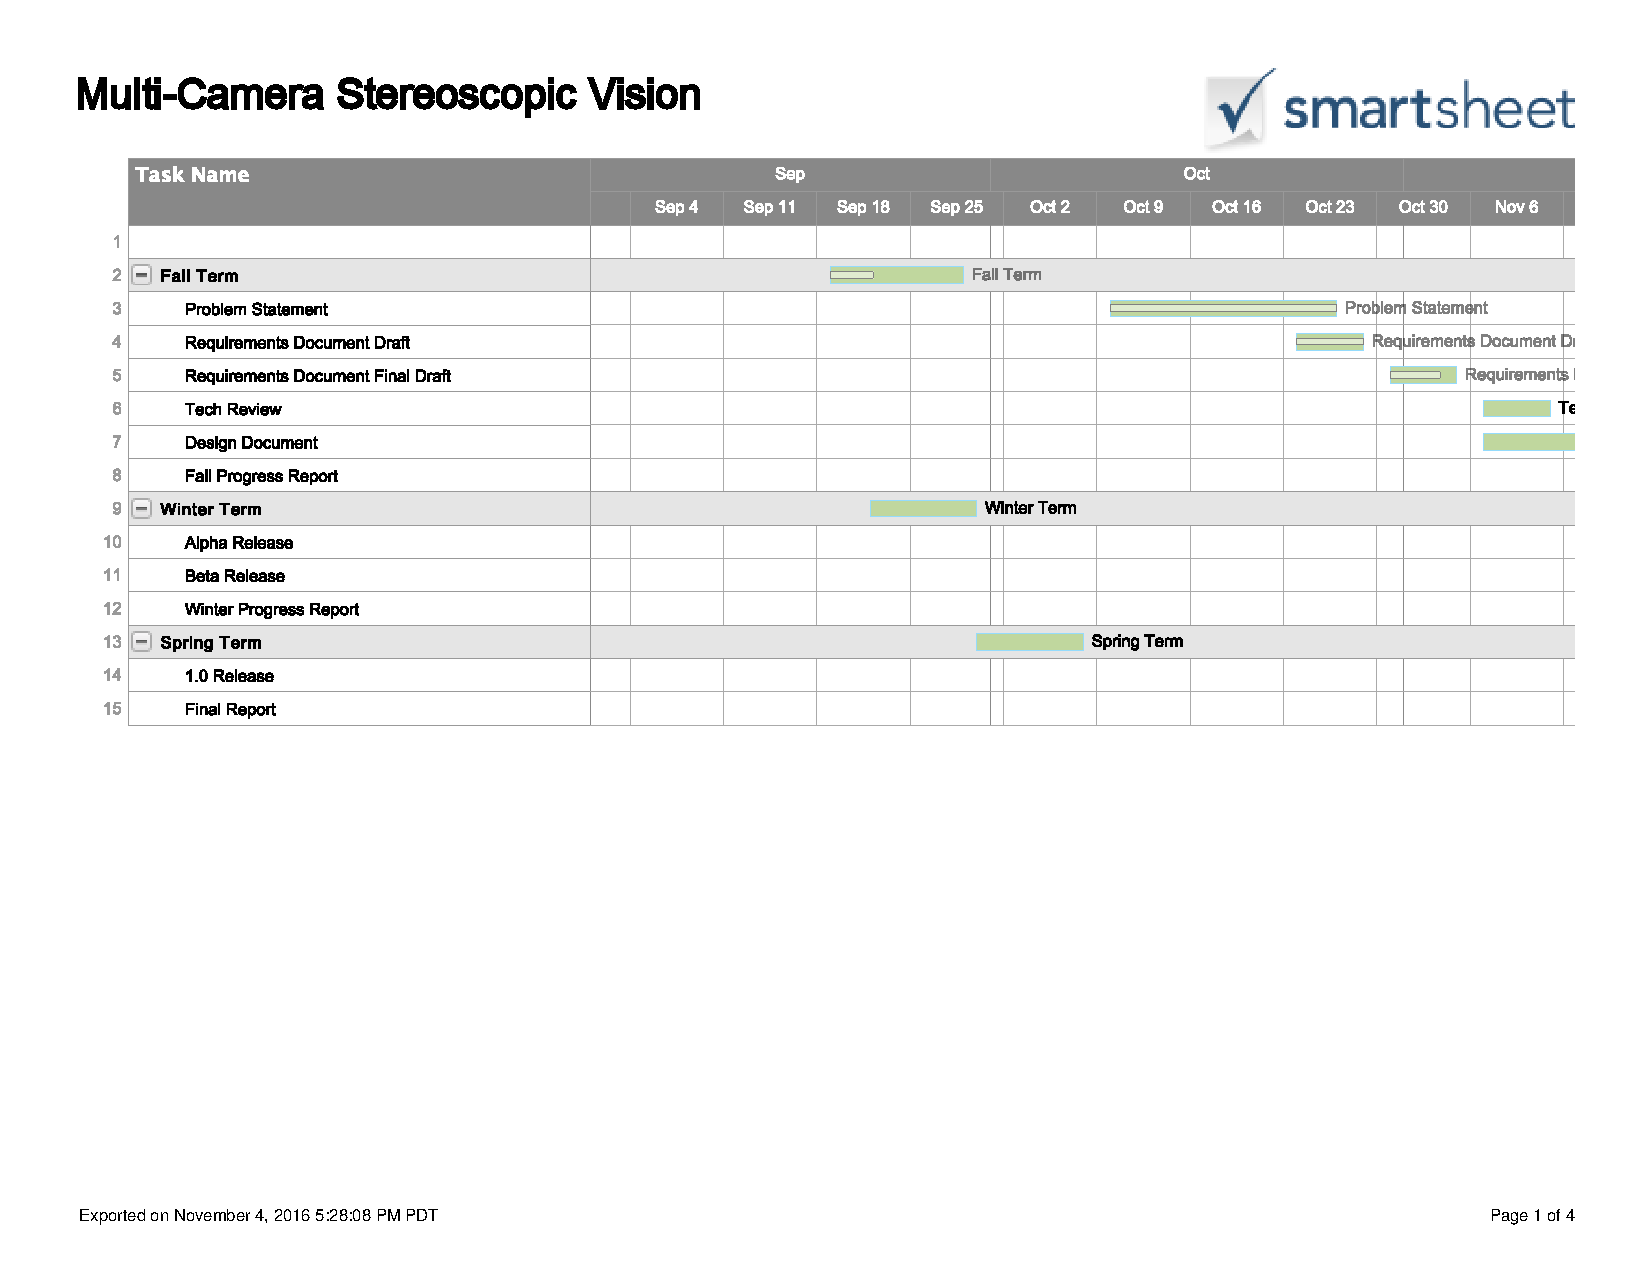
\includepdf[pages={1-3}]{rd.pdf}

\section{Specific Requirements}
\subsection{External Interfaces}
The system will only have a single external interface which will be the user’s uploaded camera files (video + metadata).
These will be processed and saved internally under the context of the application.
The process BLOB function will intake part of this data (the metadata), transform it, and save it either in memory or to a file awaiting use.
The process video file function will make use of the actual video data from the camera along with the processed BLOB data generated from the process BLOB function.

\subsection{Functions}

\subsubsection{Upload Video Files}
The system will allow users to upload two video files along with their relevant video metadata

\subsubsection{Process BLOB}
The cameras being used for this project output a video file in a BLOB, this process will be responsible for reading that BLOB and transforming it into a file type that our application can read. This will most likely be a JSON or CSV format. This functionality should also save this data either in memory or in a file, depending on the use case, so it can be later accessed.
\subsubsection*{Validity checks on the inputs}
BLOB should be in expected format
\subsubsection*{Exact sequence of operations}
\begin{enumerate}
  \item Open file pointer
  \item Validate input file
  \item Apply decoding algorithm to file contents
  \item Validate Results
\end{enumerate}
\subsubsection*{Validity checks on outputs:}
Output file should have the following: Longitude, Latitude, Timestamp, Velocity
\subsubsection*{Responses to abnormal situations}
\begin{itemize}
  \item Overflow: File too large
  \item Communication facilities: Through application provide error message to user describing the problem and what if anything they can do to remedy the situation.
  \item Error handling and recovery: If possible wait for user to fix the problem otherwise cancel process
\end{itemize}
\subsubsection*{Relationship of outputs to inputs}
The input of the function should contain the same data as the output, but decoded so that it is processable by the rest of our application. The output from this function feeds into the input of parses converted BLOB.
\subsubsection*{Video Quality Assurance}
The system will provide video processing functionality that improves quality of given video. This should include video stabilization which follows our video stabilization requirements.
\subsubsection*{Correlate video files: }
The system will synchronize the two video files such that each frame are playing nearly simultaneously. This process should also involve FOV correction between the two video files.
\subsubsection*{Convert the two processed files into a single stereoscopic video file}
The system will output a processed and correlated video file which can be viewed in a 3D capable device.

\subsubsection{Parse Converted BLOB}
\subsubsection*{Validity checks on the inputs}
Make sure decoded blob is in correct format
\subsubsection*{Exact sequence of operations}
\begin{enumerate}
  \item Read decoded BLOB from file or memory
  \item Iterate over decoded BLOB
  \item Return specific decoded BLOB information based on request
\end{enumerate}
\subsubsection*{Responses to abnormal situations}
\begin{itemize}
  \item Overflow: If the video file is too large, the file will be cut off at 2 GB, and will start a new file containing the next frames in the sequence.
  \item Communication facilities: If running in background, push notifications. If running in foreground, on screen notifications in app.
  \item Error handling and recovery: If error is non-recoverable, report why to user. If error is recoverable prompt user to take action if necessary, otherwise attempt alternative operation
\end{itemize}
\subsubsection*{Relationship of outputs to inputs}
Accepts decoded BLOB from Convert BLOB to parsable format function.
Outputs specific metadata information about frame (e.g. gps data, frame number, etc.)

\subsection{Performance Requirements}
The system should be able to process no less than 10 frames per second.
This means that given 10 minutes of 60fps video, it should take no more than 60 minutes to perform each operation to transform the video into the proper format.

\subsection{Design Constraints}
\subsubsection{Standards Compliance}
User Interface: Our desktop application should follow standard Windows/Mac design requirements/best practices.

\subsection{Software System Attributes}
\subsubsection{Reliability}
Given two camera generated video files that are able to be correlated, the system should not fail.
The system will expect the following requirements:
\begin{enumerate}
  \item The BLOBs associated with the video files will be in an expected format
  \item The two video files are capable of being correlated
  \item Video can be stabilized
  \item FOV of both cameras will be defined by the FOV camera angles of the cameras used, and will be within 5 degrees of each other.
  \item Cameras consistent distance apart
  \item Video taken concurrently
\end{enumerate}

\subsubsection{Maintainability}
If the BLOB format changes, the convert BLOB function should be able to change and the rest of the system remain the same.
This means all functions after converted BLOB should expect and accept a consistent format.

\subsubsection{Portability}
The application works on either a Mac or Windows laptop and doesn't require internet, so it can be used anywhere. Any UI design/code should not have to be compatible with any other system unless requirements change.

\end{document}
